\section{Introduction}
% introduce the significance of large-scale pretraining, across different fields, and point out the significance of CLIP

\begin{figure}[t] 
    \centering
    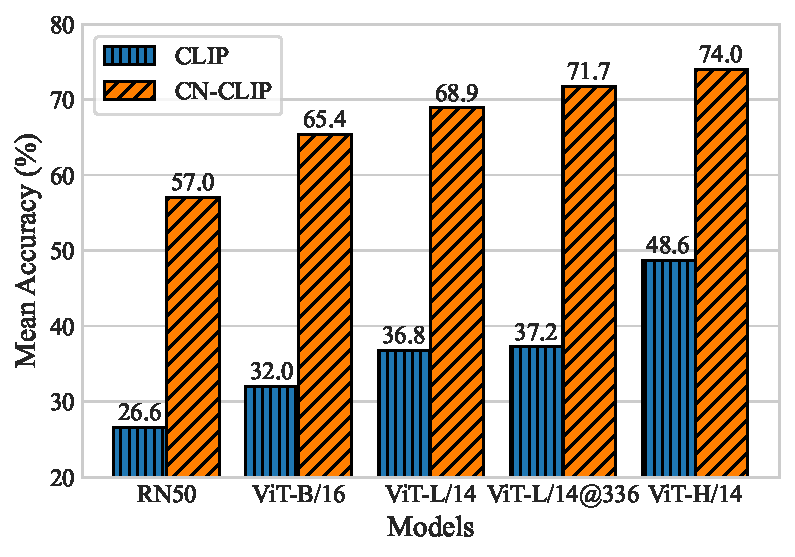
\includegraphics[width=1.0\linewidth]{pics/Mean Recall/cnclip.pdf}
    \caption{\textbf{Comparison of CLIP and Chinese CLIP models on the Chinese native retrieval benchmark MUGE.} On the benchmark based on the native data (which are mostly crawled from the language-native websites, in contrast with the translated data from websites of other countries.), CLIP performs far worse than our Chinese CLIP. Note that $\text{CLIP}\rm_{ViT\text{-}H/14}$ is not released, we use the model from OpenCLIP~\citep{openclip} instead.}
    \label{fig:comparison}
\end{figure}




Starting from the burst of pretraining in NLP, foundation models have attracted attention from multiple research communities. 
Foundation models that learn from large-scale unsupervised or weakly supervised data play as the basis of downstream models. 
% They demonstrate strong transferrability by promoting the downstream performance to a new level~\citep{bert, gpt3}. 
% A series of BERT-based models~\citep{bert, roberta, deberta} have created new state-of-the-art performance in natural language understanding~\citep{glue, superglue}, and the GPT series~\citep{gpt, gpt2, gpt3} and the following language models~\citep{lamda, palm} have demonstrated unprecedented performance in natural language generation, including text generation, dialog, etc. 
% Following natural language pretraining, the transfer of BERT~\citep{bert} and T5~\citep{t5} to multimodal pretraining was also successful~\cite{vilbert, uniter, vinvl, vilt, simvlm, ofa, beit3}. They achieved new state-of-the-art performance in multiple vision-language downstream tasks, e.g., visual question answering, image captioning, cross-modal retrieval, etc. 
% This reflects the great potential of building a foundation model pretrained on large-scale data for cross-modal representation learning. 
A milestone of foundation models~\citep{foundation_model} in multimodal representation learning is CLIP~\cite{clip}. 
Different from the conventional generative pretraining, CLIP is a contrastive-learning-based model pretrained on a large-scale dataset of around $400$ million image-text pair data collected from the web. 
Despite the simplicity of the method, CLIP not only achieved outstanding performance in vision-language retrieval but more importantly played as a vision foundation model and demonstrated state-of-the-art performance in zero-shot image classification across a series of datasets. 
% Furthermore, its simplicity facilitates its application to downstream tasks, and thus we have witnessed a series of studies following or utilizing CLIP, e.g., DALL-E~\cite{dalle, dalle2}, ViLD~\citep{vild}, StyleCLIP~\citep{styleclip}, SLIP~\citep{slip}, CLIP4Clip~\citep{clip4clip}, etc. 
CLIP which builds a connection between vision and language has been transforming the research in both multimodal representation learning and computer vision. 

Be that as it may, it is difficult to efficiently transfer a cross-modal pretrained model to another language for several causes. 
First, learning to model the distribution of language-native vision and language data is significant for the transfer. 
Though CLIP performs as a strong foundation model in most scenarios, we find that it is hard for CLIP with machine translation to perform well on the Chinese-native cross-modal retrieval benchmark.
Figure~\ref{fig:comparison} demonstrates large performance gaps between the original CLIP and our Chinese CLIP at all model scales. 
We assume that it is crucial for both encoders to learn from the language-native images and texts. 
Second, the performance of previous methods for Chinese multimodal pretraining has been inhibited by several factors. Pretraining from scratch requires collecting a large-scale quality language-specific image text pair dataset similar to Web Image Text (WIT) for OpenAI CLIP~\citep{wenlan, r2d2}. Though the fast transfer of CLIP to Chinese data can be realized by using CLIP initialization and Locked-Image Tuning~\citep{lit}, the vision encoder still cannot learn the information of images from the language-specific domains~\citep{wukong}. 
% For example, the Chinese-native data, including both the images and texts crawled from the Chinese websites, reflect information about local features, e.g., cultural values, social customs and landscapes, etc. 

% we find that it is difficult to directly transfer CLIP to language-specific scenarios, say multimodal applications in Chinese, where the data are mostly Chinese-native. 
% A very recent work is mCLIP~\citep{mclip}, which realizes multilingual CLIP by building language-specific text encoders whose output features resemble that of CLIP by training with MSE loss. 
% However, its search engine\footnote{\url{https://rom1504.github.io/clip-retrieval}} fails to return the correct results for the search queries unique to Chinese culture, e.g., ``Spring Festival couplet''. 
% We assume that vision-language foundation models should model the data distribution of the language-specific data so as to transfer to another language. 
% For example, the Chinese-native data, including both the images and texts crawled from the Chinese websites, reflect information about local features, e.g., cultural values, social customs and landscapes, etc. 

Therefore, we propose Chinese CLIP, a language-specific vision-language foundation model pretrained on the publicly available Chinese image-text pair data.  
Additionally, we still use the same architecture as OpenAI CLIP.  
To realize efficient transfer of cross-modal foundation model to Chinese data, we develop a two-stage pretraining method, which is also adaptive to other vision-language foundation models, e.g., ALIGN, Florence, etc. 
Here in this work, we use CLIP as an example. 
To be specific, we first initialize both encoders with pretrained models, namely vision encoders from CLIP and text encoders from RoBERTa-wwm-Chinese~\citep{wwm}. In Stage 1, we freeze the image encoder and only optimize the text encoder with LiT, and in Stage 2, we train both encoders with contrastive tuning~\ref{fig:model}. 
In this way, the new model can inherit from the foundation models through initialization and LiT, and effectively transfer to language-specific data through contrastive tuning. 

% Our ablation study shows that it can achieve improved model performance compared with the other pretraining options. 
We evaluate Chinese CLIP on $3$ Chinese cross-modal retrieval datasets, including MUGE\footnote{\url{https://tianchi.aliyun.com/muge}}, Flickr30K-CN~\citep{flickr30k-cn}, and COCO-CN~\citep{coco-cn}. Experimental results demonstrate that both the large-size and huge-size Chinese CLIP reach state-of-the-art performance on the $3$ datasets in the setups of both zero-shot learning and finetuning. 
Additionally, we evaluate the capability of zero-shot image classification on the track ``Image Classification in the Wild'' of the ELEVATER benchmark~\citep{elevater}. 
% Specifically, we transform the datasets with manual translation for the evaluation of Chinese models.
% \footnote{We will soon release the datasets and templates for prompt ensembling.} 
On the classification datasets, Chinese CLIP demonstrates competitive performance in comparison with state-of-the-art methods and outperforms the Chinese baselines. 
Furthermore, we provide NVIDIA TensorRT and ONNX models for deployments, which run around $2$ to $10$ times faster than Pytorch models for inference. 


% It is pretrained with our proposed two-stage pretraining method on a  large-scale Chinese image-text pair dataset
% We hypothesize that the transfer to language-specific data should significantly boost the performance on the Chinese-native benchmark. 
% Figure~\ref{fig:comparison} shows the performance of CLIP and Chinese CLIP models on MUGE Retrieval, a Chinese-native E-commerce cross-modal retrieval dataset. 
% Note that we apply CLIP by translating texts to English with the in-house automatic translation system. 
% We show that at all model scales, the gaps between CLIP and Chinese CLIP are saliently large. 
% This should be evidence that it is insufficient for the incorporation of a language-agnostic vision-language model and automatic translation to support the cross-modal applications highly relying on language-native data. 
% However, it is still a pity that there is no such model that strictly follows the design of CLIP in the community of Chinese multimodal representation learning. 
% Previous Chinese multimodal pretrained models are mainly generative multiomodal pretrained models~\citep{m6, m6-t, m6-10t}, or contrastive-learning-based models with additional complex model and training task designs~\citep{wenlan, wukong, r2d2}. 
% We assume that it is sufficient for the simple implementation of CLIP on large-scale Chinese data to achieve satisfactory performance in downstream tasks, and we are convinced that the simple architectural design of CLIP is essential to the application of multimodal pretrained models in real-world scenarios. 

% Chinese CLIP models are pretrained on large-scale Chinese image-text pair data. 
% Specifically, we construct a dataset of nearly $200$ million image-text pairs, most of which are publicly available data. 
% To improve the pretraining efficiency and downstream performance, we propose a two-stage method that effectively leverages the existent foundation models. 
% which are retrieved from: the Chinese data in LAION-5B~\citep{schuhmann2021laion}, the Wukong dataset~\citep{wukong}, translated image-text pairs from the publicly available English datasets, and an in-house dataset crawled from the Chinese websites. 
% We build $5$ Chinese CLIP models, ranging from $77$ to $958$ million parameters. 
% which are a tiny-size model with ResNet-50~\citep{resnet} and RBT3~\citep{wwm}, a base-size model with ViT-B/16~\citep{vit} and RoBERTa-wwm-Base~\citep{wwm}, two large-size models with ViT-L/14 and RoBERTa-wwm-Base pretrained on images of $224 \times 224$ and $336 \times 336$ respectively, as well as a huge-size model with ViT-H/14 and RoBERTa-wwm-Large. 
% For the pretraining, we implement a two-stage pretraining method. 

% Also, the tiny-size Chinese CLIP can significantly outperform the large-size baseline. 
% This reflects the potential of the simple architecture and pretraining on large-scale data. 

In brief, our contributions are:
\begin{itemize}
    \item We propose Chinese CLIP, a simple implementation of CLIP pretrained on our collected large-scale Chinese image-text pair data, and we propose a two-stage pretraining method to achieve high pretraining efficiency and improved downstream performance.
    \item Chinese CLIP achieves state-of-the-art performance in cross-modal retrieval in the setups of zero-shot learning and finetuning, and competitive performance in zero-shot image classification. 
    % \item We develop a series of analyses to show the effectiveness of our pretraining method and figure out the inherent problems of Chinese CLIP, e.g., sensitivity to manual prompts, inability to understand negation, etc. 
\end{itemize}
% In the following sections, we introduce the detailed implementation of Chinese CLIP and illustrate the experimental results and analyses of the model. Finally, we review the related work, point out our limitations, and conclude the paper. 
% We believe that the increases in data and model scale can further level up the downstream performance as well as the transferrablity. 
